\documentclass[conference]{IEEEtran}
\IEEEoverridecommandlockouts
% The preceding line is only needed to identify funding in the first footnote. If that is unneeded, please comment it out.
\usepackage[brazil]{babel}
\usepackage[utf8]{inputenc}
\usepackage[T1]{fontenc}
\usepackage{cite}
\usepackage{amsmath,amssymb,amsfonts}
\usepackage{algorithmic}
\usepackage{graphicx}
\usepackage{textcomp}
\usepackage{xcolor}
\def\BibTeX{{\rm B\kern-.05em{\sc i\kern-.025em b}\kern-.08em
    T\kern-.1667em\lower.7ex\hbox{E}\kern-.125emX}}
\begin{document}

\title{Aplicação do Modelo CBR para Identificação de Podócitos em Imagens Histológicas Renais Baseado em Informações de Textura\\
	\thanks{}
}

\author{\IEEEauthorblockN{\textsuperscript{} George Oliveira Barros}
	\IEEEauthorblockA{\textit{Programa de Pós-Graduação em Informática} \\
		\textit{Universidade de Brasília }\\
		Brasília, Brasil\\
		george.barros@ifgoiano.edu.br}
}

\maketitle

\begin{abstract}
Este trabalho é um relatório prático que descreve a aplicação do modelo de Raciocínio Baseado em Casos (CBR) para encontrar similaridade entre conjunto de dados de textura de amostras de imagens de podócitos. Esta atividade é um componente avaliativo da disciplina Inteligência Artificial 2, ministrada pelo professor Li Weigang, no Programa de Pós-Graduação em Informática (PPGI) da Universidade de Brasília (UNB). A ferramenta utilizada para aplicar o modelo CBR aos dados, foi o framework JColibri. Infelizmente, no final da aplicação alguns erros foram gerados no software. Portanto o relatório descreve as etapas realizadas com sucesso. 
\end{abstract}

\begin{IEEEkeywords}
Relatório, JColibri, CBR, Imagens histológicas
\end{IEEEkeywords}

\section{Apresentação do Problema e Conjunto de Dados}
As glomerulopatias são uma família de patologias renais que acometem os glomérulos, que, por sua vez, são estruturas biológicas renais responsáveis pela filtragem do sangue. O procedimento mais importante para realização do diagnóstico médico das glomerulopatias é a análise de imagens histológicas renais dos glomérulos. As imagens histológicas são adquiridas através de exame de biópsia. Após a extração de um pedaço do tecido renal, imagens de glomérulos são obtidas através de fotos realizadas por câmeras acopladas em microscópio. 

Existem uma série de padrões de lesões histológicas e a identificação de conjuntos específicos dessas lesões possibilitam aos patologistas a classificação correta do tipo de glomerulopatia presente em um glomérulo. Há uma série de tarefas que se automatizadas, ajudariam demasiadamente os patologistas, como é o caso da identificação automática dos podócitos em imagens de glomérulos. Isto ofereceria aos patologistas uma identificação mais eficiente das lesões nos podócitos e consequentemente na tarefa de classificação de glomerulopatia. 

Neste trabalho, foi utilizado um conjunto de dados extraídos de imagens de podócitos e células normais. Foi aplicado o algoritmo GLCM em 19 mil imagens de podócitos e demais células. Através do algoritmo GLCM foi extraída informações de textura com o objetivo de discriminar imagens de podócitos renais de imagens das demais células internas dos glomérulos. Deste modo, foi montado um conjunto de dados no formato .CSV contendo para cada uma das 9 mil imagens as seguintes informações: label (1 ou 0), contrast, dissimilarity, homogeneity, ASM, energy e correlation. O campo label armazena dados do tipo inteiro (1 ou 0) e diz respeito a informação de que uma determinada amostra é um podócito (1) ou não (0). Os demais campos armazenam dados decimais normalizados entre 0,0 e 10,0. 

\section{CBR e JColibri}
O Raciocínio Baseado em Casos (RBC) é um modelo empregado na área de Inteligência Artificial que utiliza dados históricos (exemplos já experimentados) como parâmetro de decisão para novos casos. Por exemplo: Ao atender um novo paciente e escutar seus problemas, o médico deve se lembrar do histórico da doença de um outro paciente devido ao conjunto similar de sintomas, e aplica a esse novo paciente um tratamento semelhante ao que administrou ao paciente que apresentou aqueles sintomas similares. E outro exemplo, um advogado deve reforçar os seus argumentos com jurisprudências semelhantes \cite{ref1}.

As aplicações do RBC são inúmeras: Algumas delas são, tarefas de classificação, síntese, diagnóstico, suporte a decisões, configuração, planejamento e projeto. Nas tarefas de classificação o é classificar (discriminar) uma amostra em um contexto específico em detrimento de outras amostras. Em aplicações de classificação, um problema é descrito por meio de um conjunto de sintomas ou observações e da solução para o problema; assim, o resultado da classificação é a seleção de uma ou mais classes ou categorias nas quais o problema poderia ser classificado. Neste caso, usualmente, as opções de classificação são realizadas dentro de um domínio qualitativo e não quantitativo. O trabalho de \cite{ref2} é um exemplo de aplicação do RBC para classificação de imagens histológicas renais em combinação com redes neurais convolucionais.

Os elementos básicos de um sistema de RBC são: Representação do conhecimento, medida de similaridade, adaptação e aprendizado. Na representação do conhecimento, o conhecimento é representado principalmente em forma de casos que descrevem experiências concretas. Por exemplo, casos abstratos e generalizados, tipos de dados, modelos de objetos usados como informação.  Na medida de similaridade o objetivo é encontrar um caso relevante para o problema atual na base de casos e responder à pergunta quando um caso relembrado for similar a um novo problema. Na adaptação, a ideia é que situações passadas representadas como casos, dificilmente serão idênticas às do problema atual. Por fim, no aprendizado, para que um sistema se mantenha atualizado e evolua continuamente, sempre que ele resolver um problema com sucesso, deverá ser capaz de lembrar dessa situação no futuro como mais um novo caso.

Há diferentes softwares que possibilitam a aplicação do modelo CBR. O JCOLIBRI é um desses softwares. O JCOLIBRI é um framework construído sob o paradigma orientado a objetos, na linguagem Java, podendo ser especializado para a construção de aplicações customizadas \cite{ref3}.

\section{Utilizando o JCOLIBRI: Classificação de Dados de Imagens de Podócitos}
A primeira tarefa a ser executada na utilização do JCoilbri é a criação de um novo projeto. A versão do JColibri instalada nesta prática foi o complemento para o IDE Eclipse disponível no site oficial do framework. Ao criar um novo projeto, entre as opções listadas a escolhida foi New CBR Project (ver Figura 1). A tarefa seguinte foi escolher as etapas de implementação do sistema. As etapas dizem respeito aos passos de implementação do CBR. Todas as opções foram mantidas.

\begin{figure}[htbp]
	\centerline{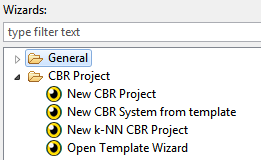
\includegraphics{fig1.png}}
	\caption{Criação do projeto.}
	\label{fig1}
\end{figure}
Em seguida a tarefa foi criar ou importar os casos base seguindo os padrões do JCOLIBRI (ver Figura 2). Neste exemplo, os dados importados foram dados decimais extraídos previamente de imagens de podócitos e outras células. Primeiro foi necessário informar a estrutura de organização dos casos, definir um identificador para os casos e enfim, importar os dados. 

\begin{figure}[htbp]
	\centerline{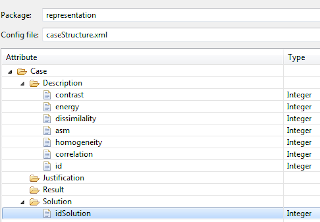
\includegraphics{fig2.png}}
	\caption{Definindo a estrutura dos casos base.}
	\label{fig2}
\end{figure}

Aqui os dados importados estavam armazenados em um arquivo . CSV, contendo 9 mil amostras. Para cada amostra, 6 atributos (incluindo 5 características de textura e o campo de rótulo das amostras, nesse caso, 1 ou 0) (ver Figura 3).
\begin{figure}[htbp]
	\centerline{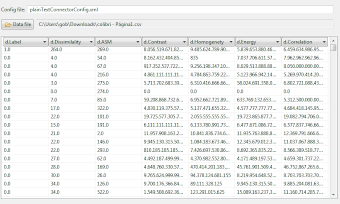
\includegraphics{fig3.png}}
	\caption{Impotando o conjunto de casos base de um aqrquivo .CSV.}
	\label{fig3}
\end{figure}

Após importar os casos base, se fez necessário escolher as medidas de similaridades e pesos para cada atributo, tarefa extremamente importante, por se tratar do método utilizado para comparar os casos históricos (casos base) com os possíveis novos casos. A medida escolhida foi o intervalo local de similaridade. O peso escolhido para todos foi 0.5 (ver a Figura 4). Este método foi o escolhido pois a ideia central do problema em questão é dado uma nova amostra descobrir se a mesma é um podócito ou não, através da análise da distância espacial da amostra nova em relação aos caso base. 

\begin{figure}[htbp]
	\centerline{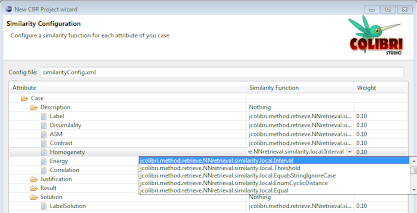
\includegraphics{fig4.png}}
	\caption{Escolha do método de cálculo de similaridade.}
	\label{fig4}
\end{figure}

A última  etapa de configuração do modelo foi a escolha da representação do catálogo do produto. A opção escolhida foi LinearCaseBase. Após a escolha o código do projeto foi gerado. Infelizmente, nessa tentativa o projeto java gerado não pôde ser executado e uma série de erros de dependências foram apontados. Na tentativa de corrigir o código, o processo de aplicação do modelo para gerar o código de maneira automática foi repetido algumas vezes. Na última tentativa o modelo de projeto JColibri escolhido foi o CBRProjectkNN. Ao utilizar essa opção o código gerado no final foi executado (ver Figur 5), no entanto, não foi possível aplicar casos novos e realizar a tarefa de classificação. O JColibri possui poucas fontes de consulta e documentação antiga e limitada. Por esses fatores não foi possível identificar os erros gerados.

\begin{figure}[htbp]
	\centerline{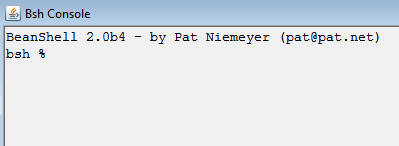
\includegraphics{fig6.png}}
	\caption{Tela de execução do projeto CBRProjectKNN.}
	\label{fig5}
\end{figure}

\section*{Código gerado}

O código gerado na última tentativa, tutoriais e artigos utilizados nesta prática encontram-se disponíveis no git-hub. Para isso basta acessar o seguinte endereço eletrônico: https://github.com/geogob/unb.


\begin{thebibliography}{00}
	\bibitem{ref1} The Cyclops Project. Raciocínio Baeado em Casos. Disponível em: http://www.inf.ufsc.br/~aldo.vw/RBC/rbc.html. Acesso em: 14 de setembro de 2019.
	
	\bibitem{ref2}  Marie, F., Corbat, L., Chaussy, Y., Delavelle, T., Henriet, J., \& Lapayre, J. C. (2019). Segmentation of deformed kidneys and nephroblastoma using Case-Based Reasoning and Convolutional Neural Network. Expert Systems with Applications, 127, 282–294. https://doi.org/10.1016/j.eswa.2019.03.010.
	
	\bibitem{ref3}  Gonz, P. A., Recio-garc, J. A., \& Antonio, A. S. (2007). Building CBR systems with j COLIBRI, 69, 68–75. https://doi.org/10.1016/j.scico.2007.02.004.
	
\end{thebibliography}

\end{document}
